\begin{exercise}
Consider the following one-dimensional \enquote{gridworld}:
You are on a route consisting of $10$ states.
The state on the left side is a terminal state with a reward of $+10$ and the state on the right is also a terminal state width a reward of $-5$.
You can move left and right.

\begin{figure}[H]
    \centering
    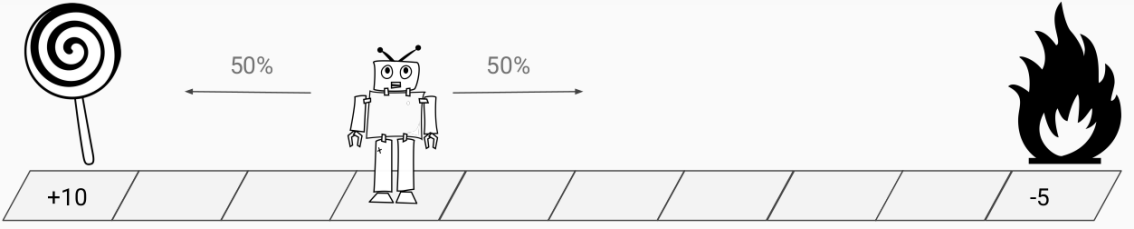
\includegraphics[width = 0.75 \textwidth]{3.24.png}
    \caption{$1$D Gridworld}
    \label{fig:3.24}
\end{figure}

Write an implementation of Dynamic Programming for estimating the values of the above states under the equiprobable random policy.

Then use policy improvement to find the optimal policy.
\end{exercise}

\begin{solution}
  See ipynb-file.
\end{solution}
